\section{Introduction}
\label{introduction}

% -----------------------------------------------------------------------------
% Finite element method.

\subsection{Finite element method}

The Finite Element Method (FEM) is a numerical technique used for finding solutions to partial differential equations as well as to integral equations. Traditional finite element methods (FEM) requires meshing techniques that generate discrete representation of potentially complex geometry. Difficulties arise when using the traditional FEM for analyzing fracture mechanics: under traditional FEM, introducing a discontinuity in the mesh, changing the material topology or drastically changing the shape of the material requires a new mesh to ensure that the element edges align with the discontinuity \citep{AH:08}. The process is laborious and difficult \citep{ZTZ:05}. The eXtended Finite Element Method (XFEM) arose as a solution to this impediment by applying enrichment functions at the position of the material interface or topology discontinuity instead of re-meshing the entire structure.

% -----------------------------------------------------------------------------
% Discontinuity

\subsection{Discontinuity}

A discontinuity can be defined as a rapid change in a field variable over a length negligible in size compared to the entire domain analyzed \citep{AH:08}. For example, in solid mechanics, strain and stress fields are discontinuous across material interfaces and displacements are discontinuous at cracks; in fluid dynamics, velocity and pressure fields are discontinuous at the boundary layer between two fluids. A discontinuity is classified as ``weak'' or ``strong''. Weak discontinuities happen when a field variable (stress field, strain rate, etc.) has a kink, meaning the derivative has a jump. This can happen at boundary layers, or at a material or fluid interface. Strong discontinuities happen when the field quantity has a jump; this could include, for example, a crack in the structure \citep{HH:04b}.

%----------------------------------------------------------------------------------------
% eXtended Finite Element Method

\subsection{eXtended Finite Element Method}

The XFEM arose as a numerical technique capable of providing local enrichment functions at the position of the material interface, avoiding the need to re-mesh the entire structure while finding solutions for the discontinuous functions \citep{FB:10}. By doing this, XFEM appears to solve the shortcomings of the FEM by providing accurate solutions for complex problems in engineering that would be impossible to solve otherwise \citep{AH:08}.

%----------------------------------------------------------------------------------------
% Level set method

\subsection{Level set method}

Level set functions are used to model the motion of these discontinuities in the elements. A level set function is a numerical scheme where the discontinuity of interest is represented as the zero level set function. Basically, a level set function has a value of zero at the boundary of its closed curve and opposite signs on the interior and the exterior (Figure \ref{fig:Level-Set}).
%
\begin{equation}
	\centering
	\begin{split}
		\phi\left(\mathbf{x}\right) > 0 & \quad \forall \mathbf{x} \in \Omega \backslash \partial \Omega \text{ (inside the region)} \\
		\phi\left(\mathbf{x}\right) = 0 & \quad \forall \mathbf{x} \in \partial \Omega \text{ (on the boundary)} \\
		\phi\left(\mathbf{x}\right) < 0 & \quad \forall \mathbf{x} \in D \backslash \Omega \text{ (outside the region)}
	\end{split}
\end{equation}
%
The XFEM uses this method by placing the discontinuity at the boundary layer and giving the interface caused by the division positive and negative values. Since the zero level is interpreted as the discontinuity, new nodes (called pseudo-nodes) are created at this position and the enrichment of the FEM is produced at this location. This creates an advantage because instead of re-meshing the entire structure, a fixed Cartesian grid is used to divide the structure and the discontinuity into domains capable of integration. Once this mesh is settled, the XFEM will subsequently use either branched or Heaviside functions to enrich the nodes and solve for the problem.
%
\begin{figure}[H]
	\centering
	\begin{tabularx}{\linewidth}{XX}
		\subfloat[]{
			\label{fig:level_set_circle_func_impl_1}
			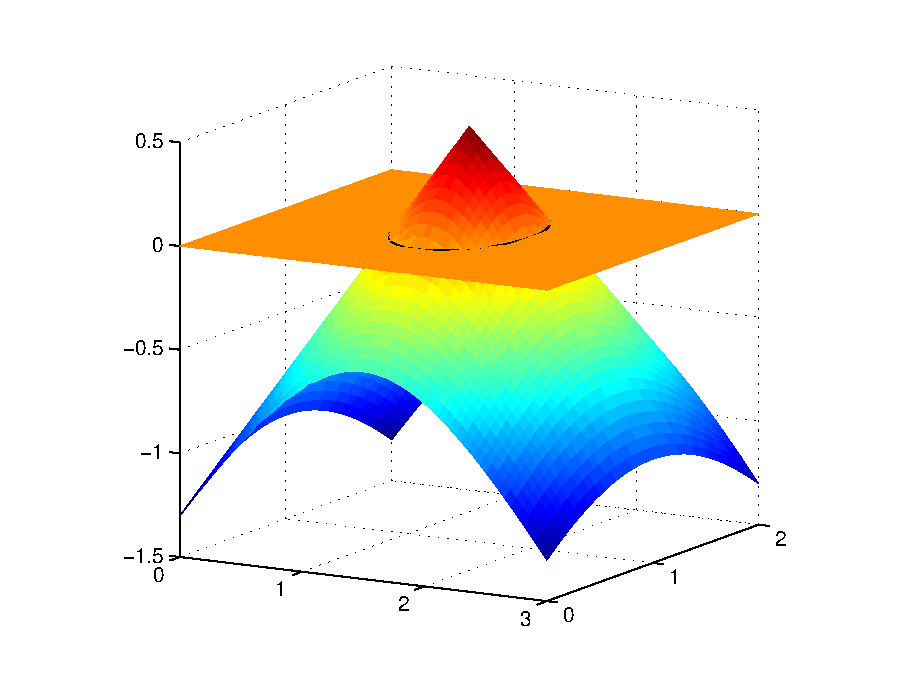
\includegraphics[width=\linewidth]{level_set_circle_func_050.eps}
		} &
		\subfloat[]{
			\label{fig:level_set_circle_domain_impl_1}
			\includegraphics[width=\linewidth]{level_set_circle_domain_050.eps}
		}
	\end{tabularx}
	\caption{The zero level set isolevel of the level set function, $\partial \Omega = \Gamma_{\phi=0}$, in \ref{fig:level_set_circle_func_impl_1} divides the fixed mesh grid into different phase regions in \ref{fig:level_set_circle_domain_impl_1}, where each phase may represent a different material or a different physics.}
	\label{fig:Level-Set}
\end{figure}

The Level Set Method (LSM) and the XFEM have a sort of natural coupling to solve problems with discontinuities. While the LSM is used to model the discontinuity and update its motion at each calculation, the XFEM is used to solve the problem and determine the direction of the discontinuity \citep{SCM+:01}.

% -----------------------------------------------------------------------------
% Delaunay triangulation

\subsection{Delaunay triangulation}

In order to apply the LSM and the XFEM to solve a problem, a framework for dividing arbitrarily complex geometries into integrable domains must be developed. The Delaunay triangulation is a critical step in this process. The Delaunay triangulation is the subdivision of a geometric object into triangles for 2D geometry and tetrahedra for 3D (Figure \ref{fig:Delaunay-Triangulation}). This particular triangulation has the property that the circumcircle of any triangle in the triangulation does not contain the vertices of other triangles or its own in its interior (Figure \ref{fig:Delaunay-Circumcircles}) \citep{LS:80}. Because triangle and tetrahedra are integrable elements, the XFEM method can then be applied.

\begin{figure}[htbp]
	\centering
		\includegraphics[width=0.75\linewidth]{delaunay_triangulation.eps}
	\caption[Delaunay triangulation]{The Delaunay formulation triangulates QUAD4 finite elements cut by the level set zero isolevel from Figure \ref{fig:level_set_circle_domain_impl_1} into TRI3 elements.}
	\label{fig:Delaunay-Triangulation}
\end{figure}

\begin{figure}[htbp]
	\centering
	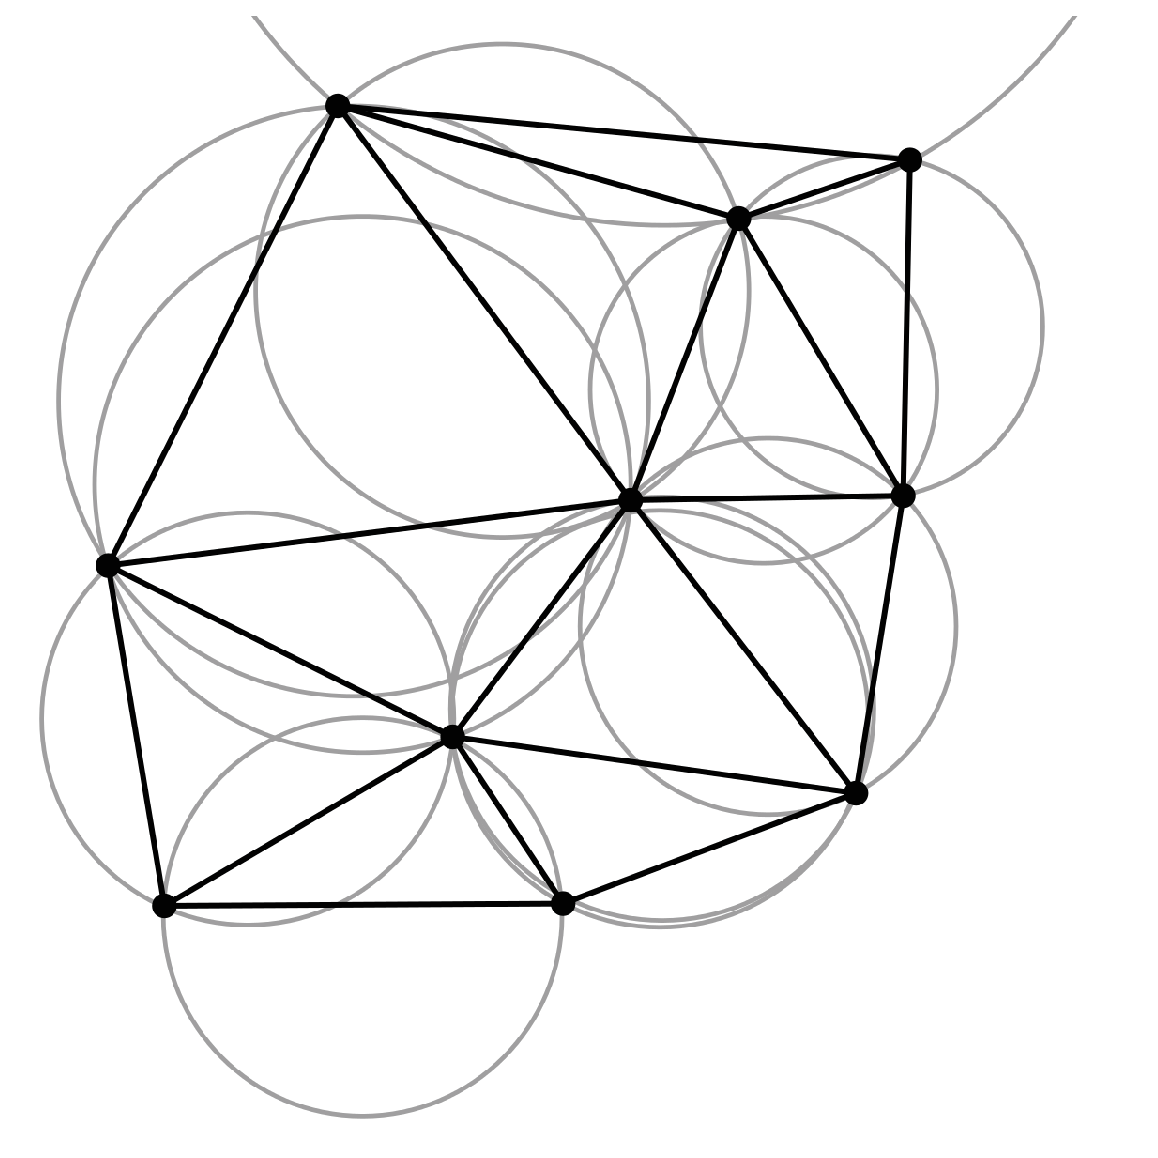
\includegraphics[width=0.5\linewidth]{delaunay_circumcircles.eps}
	\caption[Delaunay circumcircles]{Delaunay circumcircles - A set of points can be uniquely triangulated in a way that the points form circumcircles.}
	\label{fig:Delaunay-Circumcircles}
\end{figure}

For an inclusion-based XFEM model (inclusion meaning the zero level function is always a closed curve), there are only 8 triangulation configurations in 2D, while 127 different ones in 3D. Due to the low number of cases in 2D, a tabulation of the triangulation is performed instead of using the Delaunay triangulation. Figure \ref{fig:intersections_2D} shows the different cases for 2D, while Figure \ref{fig:intersections_3D} shows the triangulation of a 3D element with four different discontinuities.

\begin{figure}[htbp]
	\centering
		\includegraphics[width=\linewidth]{intersections_2D.eps}
	\caption[2D triangulation configurations]{There are only 8 different triangulation configurations for an inclusion-based XFEM model.}
	\label{fig:intersections_2D}
\end{figure}

\begin{figure}
	\centering
	\begin{tabularx}{\linewidth}{XXX}
		\subfloat[Phase ``A''.]{
			\label{fig:intersections_3D_1}
			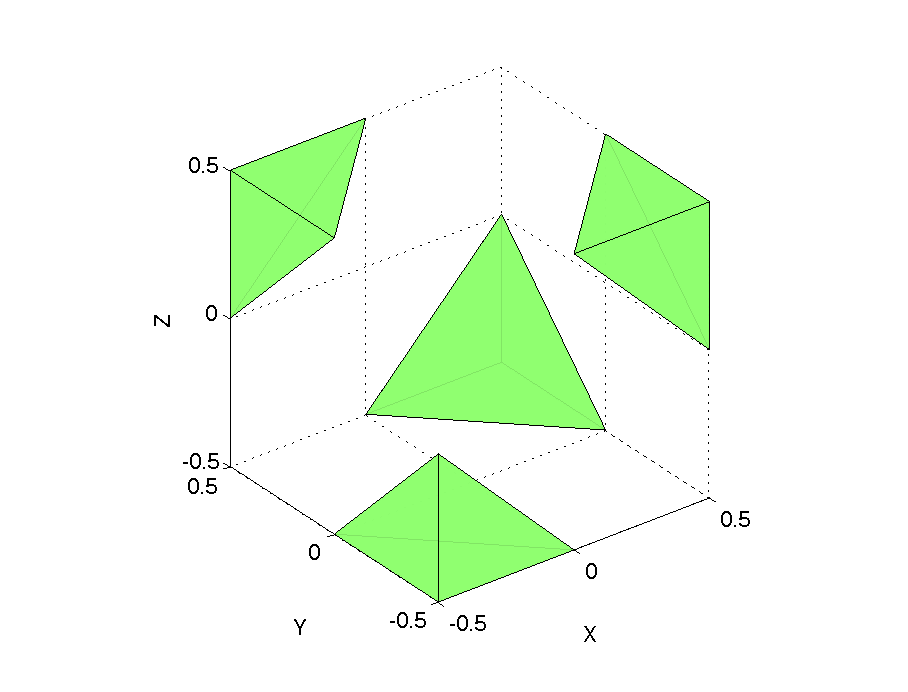
\includegraphics[width=\linewidth]{intersections_3D_1.eps}
		} &
		\subfloat[Phase ``B''.]{
			\label{fig:intersections_3D_2}
			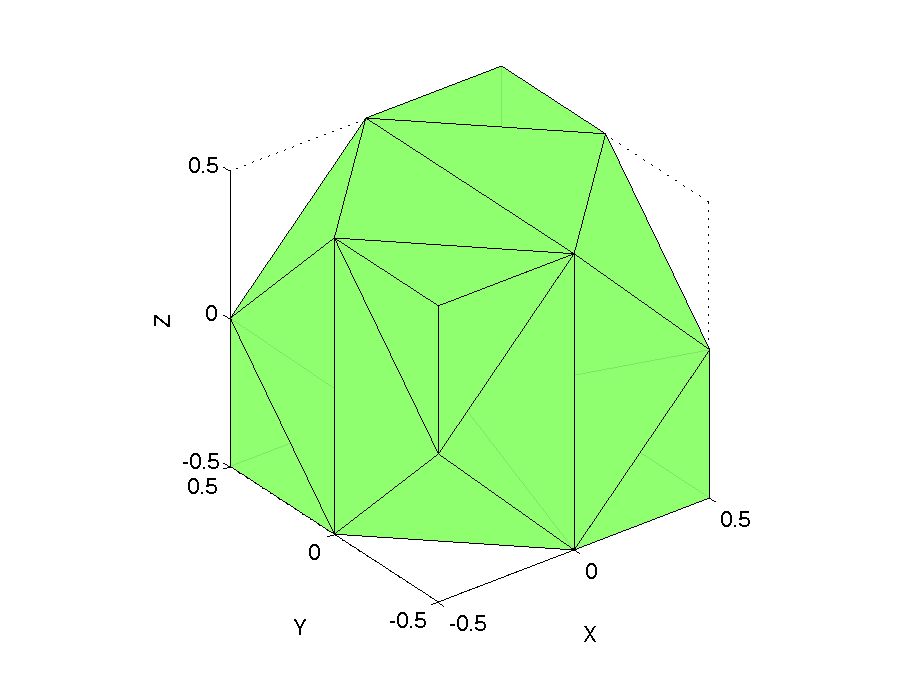
\includegraphics[width=\linewidth]{intersections_3D_2.eps}
		} &
		\subfloat[Both phase regions.]{
			\label{fig:intersections_3D_3}
			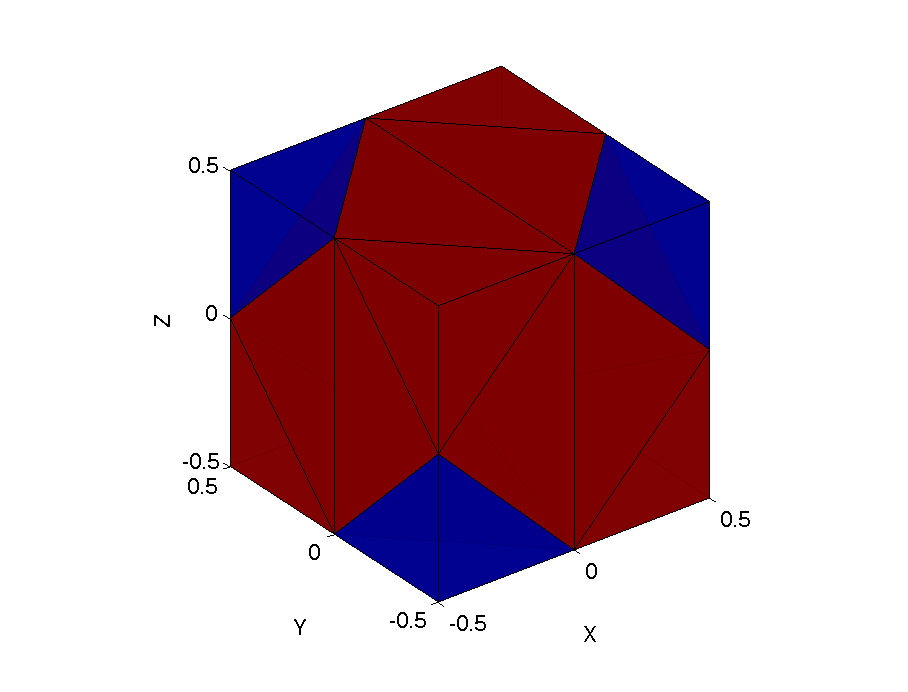
\includegraphics[width=\linewidth]{intersections_3D_3.eps}
		}
	\end{tabularx}
	\caption[3D triangulation example.]{Triangulation in 3D is more complex and we use the Delaunay triangulation algorithm to perform the computation. This element with 4 discontinuities has 4 pseudo-elements from material phase 1 and 20 from material phase 2.}
	\label{fig:intersections_3D}
\end{figure}